I dette kapitel unders�ges hvordan funktioner til videoapplikationen ville se ud, hvis ikke skulle hente deres data fra et XML dokument men i stedet hente dataene direkte fra tabeller i en relationel database. Resultatet af et funktionskald skal dog stadig v�re i form af et resultats�t beskrevet med XML.

Databasen som vil blive brugt i dette projekt er en PostgreSQL database og der arbejdes udelukkende med data fra XML dokumentet programseries.xml.

\section{Design af tabeller}

F�rste opgave er at designe nogle tabeller, som kan underst�tte indholdet i XML dokumentet. Den f�rste tabel, der skal bruges er en tabel til at holde p� selve XML dokumentet i sin komplette tilstand.  Til det form�l er tabellen �downloadedXML� oprettet. Denne tabel indeholder to kolonner, en til navnet p� XML dokumentet (docmentTitle) og en til selve indholdet af dokumentet (documentContent) som er af typen XML.

Fra unders�gelsen af programseries.xml, tilbage i kapitel 2.2, er det allerede kendt at der findes en 0 til mange relation imellem en programserie og programseriens labels, alts� kategorier. I figur \ref{postgresql:ER-diagram} ses et ER-diagram, som viser denne relation.  Derfor er der oprettet en tabel udelukkende til labels og en tabel udelukkende til indholdet af en programserie. Til at beskrive relationen, at en programserie har 0 til mange label�s og at label�s har 0 til mange programserier, s� er der oprettet en tabel, som hedder slugLabel, der har en reference til label tabellen og en reference ti l programserie tabellen. Dermed en denne relation beskrevet i databasen og tabellerne er nu klar til at indl�st data i sig.

\begin{figure}[ht]
  \centering
   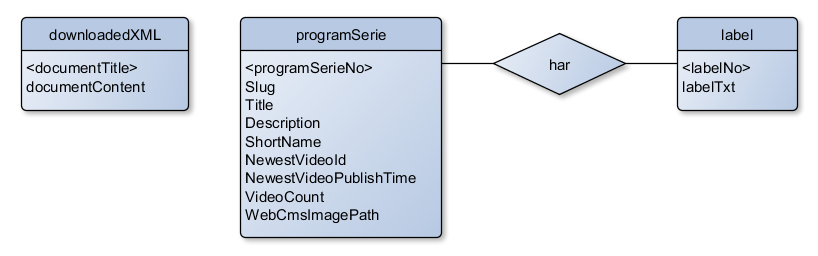
\includegraphics[width=1.1\textwidth]{pic/ER_programserie.png}
   \caption{ER-diagram over tabel-design.}
   \label{postgresql:ER-diagram}
\end{figure}

\section{Oprettelse af label�s}

N�r XML dokumentet er indl�st i tabellen downloadedXML, s� skal der som det f�rste oprettes labels til alle de kategorier, som findes i dokumentet programseries.xml. Til dette form�l er funktionen � getAndInsertAllLabels()�, som ses i figur \ref{ code: getAndInsertAllLabels} skabt. Denne funktion benytter et XPath-udtryk til at finde alle tekster til labels og for hver tekst den finder, s� unders�ges det om der allerede er oprettet en label med den tekst, hvis ikke s� inds�ttes denne nye label i tabellen. 

\begin{figure}[h]
\centering
\begin{BVerbatim}
  labels := (SELECT xpath('//ProgramSerie/Labels/string/text()', 
             downloadedXML.documentContent) FROM downloadedXML);
  FOR i IN array_lower(labels, 1) .. array_upper(labels, 1)
  LOOP
    SELECT labelNo INTO v_found FROM label WHERE label.labelTxt = labels[i];
    IF v_found IS NULL THEN
      INSERT INTO label(labelTxt) VALUES(labels[i]);
    END IF;
  END LOOP;
\end{BVerbatim}
\caption{Udsnit af funktionen getAndInsertAllLabels()}
\label{code: getAndInsertAllLabels }
\end{figure}

\section{Oprettelse af programserier samt label relationer}

For at identificere alle programserier, s� er funktionen �getAndInsertAllSlugs()� implementeret. Denne funktion finder med et XPath-udtryk alle programseriers \ele{slug} tag�s indhold og sender det videre til funktionen �getAndInsertSlugsDetail()�, som har til opgave et hente detaljerne ud og oprette relationer imellem programserierne og deres eventuelle label�s. Denne funktion ses i figur \ref{code:getAndInsertSlugsDetail}

\begin{figure}[h]
\centering
\begin{BVerbatim}
CREATE OR REPLACE FUNCTION getAndInsertSlugsDetail(p_slug VARCHAR) RETURNS VARCHAR AS $$
<< outerblock >>
DECLARE
  v_title                   text;
  v_description             text;
  v_shortName               text;
  v_newestVideoId           integer;
  v_newestVideoPublishTime  timestamp without time zone;
  v_videoCount              integer;
  v_webCmsImagePath         text;
  v_tag_value               text[];
  v_labels                  text[];
  v_programSerieNo          integer;
  v_labelNo                 integer;
BEGIN
  v_tag_value := (SELECT xpath('//ProgramSerie[Slug='''|| 
                  p_slug ||''']/Title/text()', 
                  downloadedXML.documentContent) FROM downloadedXML);
  v_title := v_tag_value[1];
  v_tag_value := (SELECT xpath('//ProgramSerie[Slug='''|| 
                  p_slug ||''']/Description/text()', 
                  downloadedXML.documentContent) FROM downloadedXML);
  v_description := v_tag_value[1];
  /**********************************************************/
  /* ...... samme metode for resten af variabelerne ....... */
  /**********************************************************/
  v_tag_value := (SELECT xpath('//ProgramSerie[Slug='''|| p_slug 
                  ||''']/WebCmsImagePath/text()', 
				  downloadedXML.documentContent) FROM downloadedXML);
  v_webCmsImagePath := v_tag_value[1];    
  INSERT INTO programSerie (Slug, Title, Description, ShortName, NewestVideoId, 
                            NewestVideoPublishTime, VideoCount, WebCmsImagePath)
  VALUES (p_slug, v_title, v_description, v_shortName, v_newestVideoId, 
          v_newestVideoPublishTime, v_videoCount, v_webCmsImagePath)
  RETURNING programSerie.programSerieNo INTO v_programSerieNo;

  v_labels := (SELECT xpath('//ProgramSerie[Slug='''|| p_slug 
               ||''']/Labels/string/text()', 
               downloadedXML.documentContent) FROM downloadedXML);
  IF array_lower(v_labels, 1) IS NOT NULL THEN
    FOR i IN array_lower(v_labels, 1) .. array_upper(v_labels, 1)
    LOOP
      SELECT labelNo INTO v_labelNo FROM label WHERE label.labelTxt = v_labels[i];
      IF v_labelNo IS NOT NULL THEN
        INSERT INTO slugLabel (programSerieNo, labelNo) 
		VALUES(v_programSerieNo, v_labelNo);
      END IF;
    END LOOP;
  END IF;
  RETURN v_title;
END;
$$ LANGUAGE plpgsql;
\end{BVerbatim}
\caption{Funktionen getAndInsertSlugsDetail()}
\label{code:getAndInsertSlugsDetail}
\end{figure}
